% Generated by code/needham.py -- do not edit by hand.
\definecolor{qocA}{rgb}{0.00,0.45,0.70}
\definecolor{qocB}{rgb}{0.90,0.60,0.00}
\definecolor{qocC}{rgb}{0.00,0.62,0.45}
\definecolor{qocD}{rgb}{0.80,0.40,0.00}
\definecolor{qocE}{rgb}{0.80,0.60,0.70}
\definecolor{qocF}{rgb}{0.35,0.70,0.90}
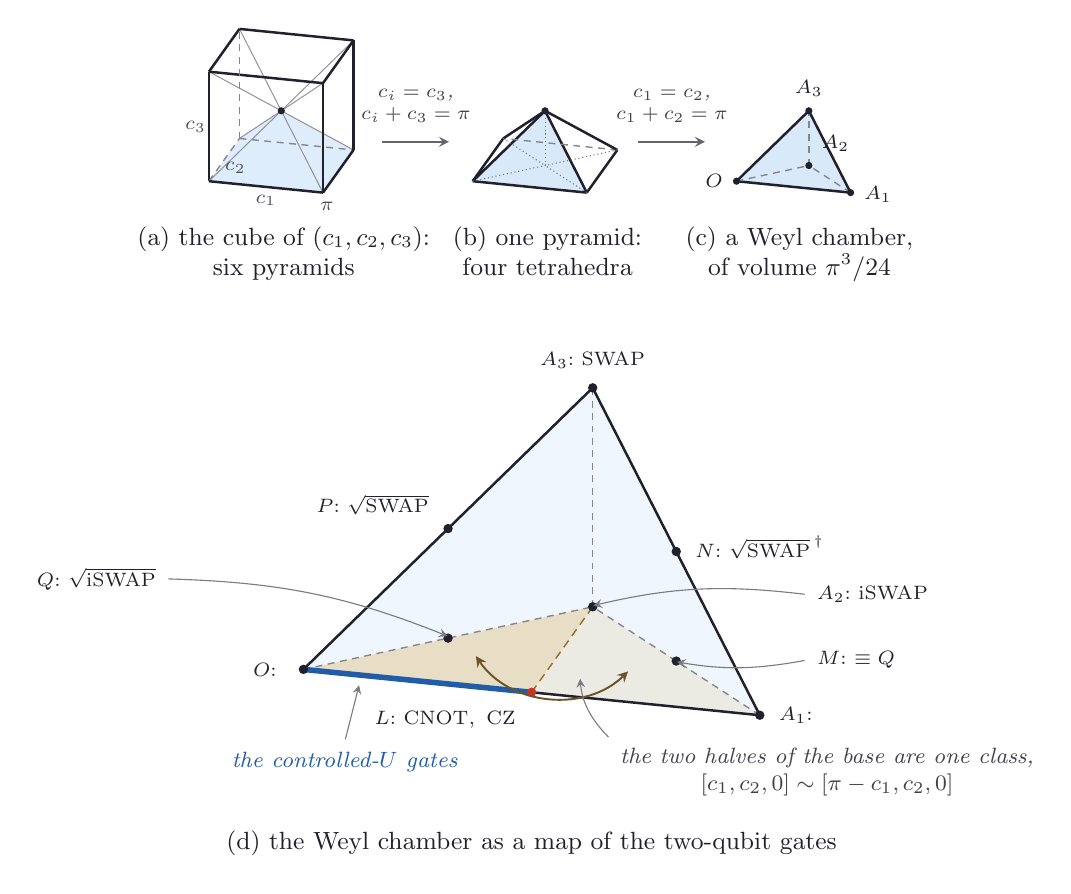
\begin{tikzpicture}[ink/.style={line width=0.9pt, ndInk}, faint/.style={line width=0.4pt, ndInk!35}, dashedink/.style={line width=0.5pt, ndInk!55, dash pattern=on 2.5pt off 2pt}, vec/.style={->, >=stealth, line width=1.2pt}, note/.style={font=\footnotesize\itshape, text=ndInk!85, align=center}, pointer/.style={->, >=stealth, line width=0.4pt, ndInk!60, shorten >=2pt, shorten <=1pt}, dot/.style={circle, fill=ndInk, inner sep=0pt, minimum size=3.4pt}, wash/.style={fill=ndSky, fill opacity=0.55}, every node/.style={text=ndInk}]
\definecolor{ndInk}{rgb}{0.13,0.13,0.18}
\definecolor{ndPaper}{rgb}{0.99,0.96,0.88}
\definecolor{ndSky}{rgb}{0.84,0.91,0.98}
\definecolor{ndRose}{rgb}{0.98,0.86,0.84}
\definecolor{ndBlue}{rgb}{0.13,0.36,0.66}
\definecolor{ndRed}{rgb}{0.78,0.20,0.16}
\definecolor{ndGold}{rgb}{0.88,0.62,0.10}
\definecolor{ndGreen}{rgb}{0.18,0.52,0.30}
\fill[ndSky, fill opacity=0.8] (1.837,6.597) -- (0.919,7.094) -- (0.388,6.743) -- (0.000,6.200) -- (1.449,6.055) -- cycle;
\draw[line width=0.35pt, ndInk!50] (0.919,7.094) -- (0.000,6.200);
\draw[line width=0.35pt, ndInk!50] (0.919,7.094) -- (0.000,7.591);
\draw[line width=0.35pt, ndInk!50] (0.919,7.094) -- (0.388,6.743);
\draw[line width=0.35pt, ndInk!50] (0.919,7.094) -- (0.388,8.134);
\draw[line width=0.35pt, ndInk!50] (0.919,7.094) -- (1.449,6.055);
\draw[line width=0.35pt, ndInk!50] (0.919,7.094) -- (1.449,7.445);
\draw[line width=0.35pt, ndInk!50] (0.919,7.094) -- (1.837,6.597);
\draw[line width=0.35pt, ndInk!50] (0.919,7.094) -- (1.837,7.988);
\draw[ink] (0.000,6.200) -- (0.000,7.591);
\draw[dashedink] (0.000,6.200) -- (0.388,6.743);
\draw[ink] (0.000,6.200) -- (1.449,6.055);
\draw[ink] (0.000,7.591) -- (0.388,8.134);
\draw[ink] (0.000,7.591) -- (1.449,7.445);
\draw[dashedink] (0.388,6.743) -- (0.388,8.134);
\draw[dashedink] (0.388,6.743) -- (1.837,6.597);
\draw[ink] (0.388,8.134) -- (1.837,7.988);
\draw[ink] (1.449,6.055) -- (1.449,7.445);
\draw[ink] (1.449,6.055) -- (1.837,6.597);
\draw[ink] (1.449,7.445) -- (1.837,7.988);
\draw[ink] (1.837,6.597) -- (1.837,7.988);
\node[dot, minimum size=2.6pt] at (0.919,7.094) {};
\node[font=\scriptsize, text=ndInk!80] at (0.724,5.957) {$c_1$};
\node[font=\scriptsize, text=ndInk!80] at (0.334,6.371) {$c_2$};
\node[font=\scriptsize, text=ndInk!80] at (-0.170,6.895) {$c_3$};
\node[font=\scriptsize, text=ndInk!80] at (1.499,5.885) {$\pi$};
\fill[ndSky, fill opacity=0.95] (3.350,6.200) -- (4.799,6.055) -- (4.269,7.094) -- cycle;
\draw[ink] (3.350,6.200) -- (4.799,6.055);
\draw[ink] (3.350,6.200) -- (3.738,6.743);
\draw[ink] (3.350,6.200) -- (4.269,7.094);
\draw[ink] (4.799,6.055) -- (5.187,6.597);
\draw[ink] (4.799,6.055) -- (4.269,7.094);
\draw[dashedink] (5.187,6.597) -- (3.738,6.743);
\draw[ink] (5.187,6.597) -- (4.269,7.094);
\draw[ink] (3.738,6.743) -- (4.269,7.094);
\draw[line width=0.4pt, ndInk!60, densely dotted] (3.350,6.200) -- (4.269,6.399);
\draw[line width=0.4pt, ndInk!60, densely dotted] (5.187,6.597) -- (4.269,6.399);
\draw[line width=0.4pt, ndInk!60, densely dotted] (4.799,6.055) -- (4.269,6.399);
\draw[line width=0.4pt, ndInk!60, densely dotted] (3.738,6.743) -- (4.269,6.399);
\draw[line width=0.4pt, ndInk!60, densely dotted] (4.269,6.399) -- (4.269,7.094);
\node[dot, minimum size=2.6pt] at (4.269,7.094) {};
\fill[ndSky, fill opacity=0.95] (6.700,6.200) -- (8.149,6.055) -- (7.619,7.094) -- cycle;
\draw[ink] (6.700,6.200) -- (8.149,6.055);
\draw[dashedink] (6.700,6.200) -- (7.619,6.399);
\draw[ink] (6.700,6.200) -- (7.619,7.094);
\draw[dashedink] (8.149,6.055) -- (7.619,6.399);
\draw[ink] (8.149,6.055) -- (7.619,7.094);
\draw[dashedink] (7.619,6.399) -- (7.619,7.094);
\node[dot, minimum size=2.6pt] at (6.700,6.200) {};
\node[font=\scriptsize, anchor=east] at (6.650,6.200) {$O$};
\node[dot, minimum size=2.6pt] at (8.149,6.055) {};
\node[font=\scriptsize, anchor=west] at (8.199,6.035) {$A_1$};
\node[dot, minimum size=2.6pt] at (7.619,6.399) {};
\node[font=\scriptsize, anchor=south west] at (7.659,6.459) {$A_2$};
\node[dot, minimum size=2.6pt] at (7.619,7.094) {};
\node[font=\scriptsize, anchor=south] at (7.619,7.154) {$A_3$};
\draw[->, >=stealth, line width=0.6pt, ndInk!70] (2.20,6.70) -- (3.05,6.70);
\node[note, anchor=south, font=\scriptsize\itshape] at (2.63,6.82) {$c_i=c_3$,\\ $c_i+c_3=\pi$};
\draw[->, >=stealth, line width=0.6pt, ndInk!70] (5.45,6.70) -- (6.30,6.70);
\node[note, anchor=south, font=\scriptsize\itshape] at (5.88,6.82) {$c_1=c_2$,\\ $c_1+c_2=\pi$};
\node[font=\small, align=center, anchor=north] at (0.95,5.75) {(a) the cube of $(c_1,c_2,c_3)$:\\ six pyramids};
\node[font=\small, align=center, anchor=north] at (4.30,5.75) {(b) one pyramid:\\ four tetrahedra};
\node[font=\small, align=center, anchor=north] at (7.50,5.75) {(c) a Weyl chamber,\\ of volume $\pi^3/24$};
\fill[ndGold!40] (1.200,0.000) -- (4.098,-0.291) -- (4.874,0.795) -- cycle;
\fill[ndGold!18] (6.996,-0.582) -- (4.098,-0.291) -- (4.874,0.795) -- cycle;
\fill[ndSky, fill opacity=0.4] (1.200,0.000) -- (6.996,-0.582) -- (4.874,3.576) -- cycle;
\draw[ink] (1.200,0.000) -- (6.996,-0.582);
\draw[dashedink] (1.200,0.000) -- (4.874,0.795);
\draw[ink] (1.200,0.000) -- (4.874,3.576);
\draw[dashedink] (6.996,-0.582) -- (4.874,0.795);
\draw[ink] (6.996,-0.582) -- (4.874,3.576);
\draw[dashedink] (4.874,0.795) -- (4.874,3.576);
\draw[line width=0.5pt, ndGold!60!ndInk, densely dashed] (4.098,-0.291) -- (4.874,0.795);
\draw[line width=2.0pt, ndBlue] (1.200,0.000) -- (4.098,-0.291);
\node[dot, fill=ndInk, minimum size=3.4pt] at (1.200,0.000) {};
\node[dot, fill=ndInk, minimum size=3.4pt] at (6.996,-0.582) {};
\node[dot, fill=ndInk, minimum size=3.4pt] at (4.874,0.795) {};
\node[dot, fill=ndInk, minimum size=3.4pt] at (4.874,3.576) {};
\node[dot, fill=ndRed, minimum size=3.4pt] at (4.098,-0.291) {};
\node[dot, fill=ndInk, minimum size=3.4pt] at (5.935,0.106) {};
\node[dot, fill=ndInk, minimum size=3.4pt] at (5.935,1.497) {};
\node[dot, fill=ndInk, minimum size=3.4pt] at (3.037,1.788) {};
\node[dot, fill=ndInk, minimum size=3.4pt] at (3.037,0.397) {};
\node[font=\scriptsize, anchor=east] at (1.080,0.000) {$O$:\ $\Id$};
\node[font=\scriptsize, anchor=west] at (7.116,-0.582) {$A_1$:\ $\Id$};
\node[font=\scriptsize, anchor=south] at (4.874,3.696) {$A_3$:\ $\mathrm{SWAP}$};
\node[font=\scriptsize, anchor=north east] at (4.018,-0.411) {$L$:\ $\mathrm{CNOT},\ \mathrm{CZ}$};
\node[font=\scriptsize, anchor=south east] at (2.917,1.838) {$P$:\ $\sqrt{\mathrm{SWAP}}$};
\node[font=\scriptsize, anchor=west] at (6.055,1.547) {$N$:\ $\sqrt{\mathrm{SWAP}}^{\,\dagger}$};
\node[font=\scriptsize, anchor=east] (lQ) at (-0.55,1.15) {$Q$:\ $\sqrt{\mathrm{iSWAP}}$};
\draw[pointer] (lQ.east) to[bend left=10] (3.097,0.397);
\node[font=\scriptsize, anchor=west] (lA2) at (7.60,0.95) {$A_2$:\ $\mathrm{iSWAP}$};
\draw[pointer] (lA2.west) to[bend right=10] (4.814,0.795);
\node[font=\scriptsize, anchor=west] (lM) at (7.60,0.12) {$M$:\ $\equiv Q$};
\draw[pointer] (lM.west) to[bend left=10] (5.875,0.106);
\node[note, anchor=north, text=ndBlue] (cu) at (1.724,-0.923) {the controlled-$U$ gates};
\draw[pointer] (cu.north) -- (1.924,-0.133);
\draw[<->, >=stealth, line width=0.7pt, ndGold!40!ndInk] (3.391,0.168) to[bend right=50] (5.323,-0.026);
\node[note, anchor=north west] (fold) at (5.098,-0.882) {the two halves of the base are one class,\\ $[c_1,c_2,0]\sim[\pi-c_1,c_2,0]$};
\draw[pointer] (fold.north west) to[bend left=20] (4.707,-0.049);
\node[font=\small, anchor=north] at (4.098,-1.932) {(d) the Weyl chamber as a map of the two-qubit gates};
\end{tikzpicture}
